\documentclass[11pt]{article}

\usepackage[utf8]{inputenc}
\usepackage{cite}
\usepackage{url}
\usepackage{graphicx}
\usepackage{caption}
\usepackage{subcaption}
\usepackage{float}
\usepackage{amsmath}
\usepackage{amsfonts}
\usepackage{amssymb}
\usepackage{algorithm}
\usepackage{algpseudocode}

\title{Foreign Exchange Rates forcasting with LSTM}
\author{Huy Phung, Tashi Choden, Sahil Pasricha
  \\University of Konstanz}
\date{February 2019}


\begin{document}

\maketitle
\pagebreak
\tableofcontents
\pagebreak

%%%%%%%%%%%%%%%%%%%%%%%%%%%%%%%%%%%%%%%%%%%%%%%%%%%%%%%%%%%%%%%%%%%%%%%%%%%%%%%%
\section{Abstract}
Foreign Exchange (abbreviation \textit{Forex} or simply \textit{FX}) Market is
the decentralized market for currency investment. Forex market is the second
most important market, after stock market. Supply and demand in the market
determine Forex rate, in which a pair of currency can be exchanged. Forex Rates
has been studied in econometrics as a financial timeseries. The purpose of
studying Forex rates is to explain the market behaviour or forecast future
prices.\\
In our project, we use statistical models and deep learning model to predict the
future rates of one step ahead. Our goal is to compare the effectiveness of LSTM
and statistical models (ARIMA and VAR) as timeseries models, in both accuracy
and performance.

%%%%%%%%%%%%%%%%%%%%%%%%%%%%%%%%%%%%%%%%%%%%%%%%%%%%%%%%%%%%%%%%%%%%%%%%%%%%%%%%

\section{Problem Description}
\subsection{Forex rates}
Foreign Exchange rates (short Forex rates) are decided solely by support and
demand of Forex market. Each rate represents the price to buy or sell a pair of
currency (e.g. EURUSD) at the moment. The price to buy is called Bid price; the
price to sell is called Ask price. The difference between Bid price and Ask
price is called Spread. In this project we consider only the Bid price. However,
if both Bid and Ask (and therefore Spread) were available, our analysis would be
more precise.\\
Forex brokers update rates according to the market within milliseconds by
standardized FIX (Financial Information eXchange) protocol. The time interval
between FIX market update messages are not uniform; it may varies from a
millisecond to few seconds. Therefore, the timeseries is of continuous time
step. In order to simplify our analysis, we convert it to a data form that has
discrete, uniform time step, while still keep important information.\\
One possible way to do so is to format the rates into OHLC format. This approach
is widely used in financial technical analysis. We partition the timeseries into
intervals of uniform time length $t$. For each interval, we keep only 4 rate:
the first (\textit{open}), the last (\textit{close}), the maximum
(\textit{high}), the minimum (\textit{low}). Since the time intervals are
uniform among dataset, we have the desired discrete, uniform time step for
analysis.

\begin{figure}
    \begin{subfigure}[b]{0.5\textwidth}
      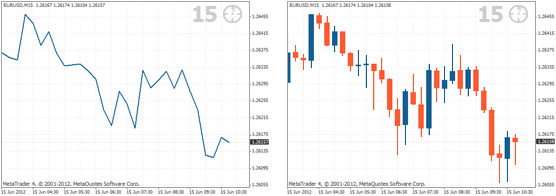
\includegraphics[height=3cm]{figs/ohlc.png}
      \caption{Original rates and OHLC form}
    \end{subfigure}
    \quad\quad\quad\quad\quad\quad\quad
    \begin{subfigure}[b]{0.2\textwidth}
      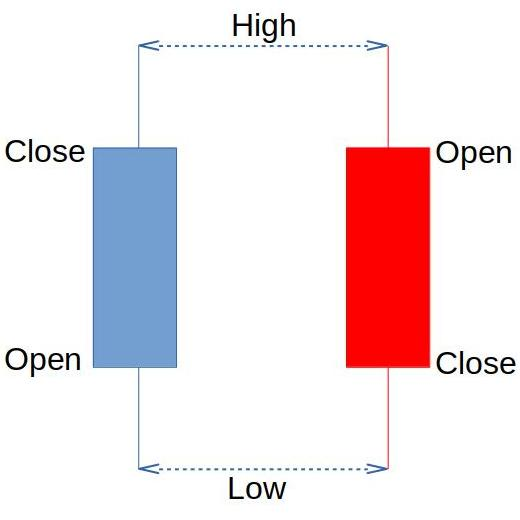
\includegraphics[height=3cm]{figs/candle.png}
      \caption{Candlestick}
    \end{subfigure}
    \caption{}
\end{figure}

\subsection{Prediction}
In this project, we concern about the prediction of future Open, High, Low,
Close prices. Other features, either originally exists (volume) or later added
(mean, median, momentum), are only considered as supporting features. These
features are only used for prediction of OHLC features.\\
The problem we are trying to solve in this project is declared as follow: given
history data in OHLC form of Forex rates, namely $x_0, x_1,\ldots,x_k$ where
$x_i=(x^O_i, x^H_i, x^L_i, x^C_i )$, predict future rate of \textit{one} step
ahead, $x_{k+1}$. 

\subsection{Dataset}
Acquiring real-time data is expensive, due to the fact that most FIX data
providers requires subscription contract. However, Janus \cite{meehau16eurusd}
collected an EURUSD rate dataset. The dataset consists of OHLC of BID price (no
ASK price) of EURUSD rates from 2010 to 2016, thus contains 245444 values. Time
interval for OHLC value is uniformly set to 15 minutes. Janus also published a
smaller sample subset of the dataset, which contains only 14880 values. We would
use the sample dataset later for ARIMA parameter search to reduce computational
effort.\\
We separate 245444 records into 3 sets: train set, validation set, test set. In
our default configuration, 80\% of the dataset is trainset (19636 records), 10\%
is valid set (2454 records), 10\% test set.\\



%%%%%%%%%%%%%%%%%%%%%%%%%%%%%%%%%%%%%%%%%%%%%%%%%%%%%%%%%%%%%%%%%%%%%%%%%%%%%%%%
\subsection{Model selection}
\subsubsection{Akaike Information Criterion (AIC)}
Akaike Information Criterion (AIC) is basically log-likelihood, but it penalizes
a model by the number of parameters. AIC is widely used in statistical model
selection, not only ARIMA and VAR, but also Hidden Markov Model and so on.
$$
AIC = 2k -2\ln(\hat{L})
$$
in which $k$ is the number of parameters and $\hat{L}$ is the likelihood. Since
the log-likelihood is multiplied by -1, lower AIC means the model fits better to
the data.

\subsubsection{Root Mean Squared Error (RMSE)}
Root Mean Squared Error is widely used to measure the difference between values
predicted by a model and the actually observed values. Given $y$ represents the
actually observed values and $\hat{y}$ represents the values predicted, $RMSE$
is given by:
$$
RMSE = \left( \frac{1}{n}\sum _{i=1}^{n}(y_i -\hat{y}_i)^2 \right)^\frac{1}{2}
$$
Root Mean Squared Error shows difference between $y$ and $\hat{y}$ regardless
the difference is negative or positive. However, since it does not take the
range of possible values into account, it would be difficult to intepret the
$RMSE$ result without knowing the possible range of predicted and actual values.

\subsubsection{Mean Absolute Percentage Error (MAPE)}
In order to measure the difference between predicted values and actual values
with regarding to the scale, we use Mean Absolute Percentage Error (MAPE)
$$
MAPE = \frac{100\%}{n}\sum  _{i=1}^{n}\left| \frac{y_i -\hat{y}_i}{y_i} \right|
$$
Compare to RMSE, MAPE is easier to interpret, for it is only a ratio without
unit. Knowing the Max-Min range of the data beforehand is not necessary. The
drawback could be the absolute value function, which is not continuous and thus
make it difficult to take it as a loss function. However, we do not use it as a
loss function here.

%%%%%%%%%%%%%%%%%%%%%%%%%%%%%%%%%%%%%%%%%%%%%%%%%%%%%%%%%%%%%%%%%%%%%%%%%%%%%%%%
\section{Statistical Models}
\subsection{Basic of Time series.}
Let $\{x_t\}$ is a timeseries with $\mu=\mu(t)$ is its mean and
$\sigma=\sigma(t)$ is its variance. \textbf{Autocovariance} of lag $k$ is
defined as $C_k=E[(x_t-\mu)(x_{t+k}-\mu)]$ and \textbf{autocorrelation} is
defined
as $\rho_k=\frac{C_k}{\sigma^2}$.\\
A time series $\{e_t\}$ is a \textit{discrete white noises} if its elements
$e_i$ are independent, identically distributed, have mean equals to zero and no
autocorrelation between any of its values. Formally,
$\mu_{\{e_t\}}=\mu_{\{e_t\}}(t)=0$,
$Cor(e_i,e_j)\neq 0, \forall i \neq j$.\\
A time series $\{x_t\}$ is a \textit{random walk} if it satisfies that
$x_t=x_{t-1}+e_t$ where $\{e_t\}$ is a discrete white noise as described above.\\
The following models we consider are similar to linear regression to some
extents. Their rationales is that we find a linear relation between the
value at time $t$ and certain \textit{lags} before it . Detailed explanation of
the models can be found at \cite{GVK483463442} and \cite{quantstart}.

\subsection{ARIMA(p,d,q)}
\subsubsection{Model description}
\textit{ARIMA(p,d,q)} consists of three models: $AR(p)$, $MA(q)$ and integrated
series of order d.\\ 
A timeseries $\{x_t\}$ is a \textit{Auto-Regression} $AR(p)$ if it satisfies that
$$
x_t = \alpha_1x_{t-1} + \ldots + \alpha_{t-p}x_{t-p} + e_t 
$$
where $\{e_t\}$ is discrete white noises. So, \textit{AR(p)} model looks back to
find a linear relation with $p$ previous values. Normally, we use
Autocorrelation Plot (ACF) of log difference to find $p$, which is the highest
lag in which we find a significant autocorrelation.\\
\\
A timeseries $\{x_t\}$ is a \textit{Moving Average} $AR(p)$ if it satisfies that
$$
x_t = \alpha_1e_{t-1} + \ldots + \alpha_{t-p}e_{t-p} + e_t 
$$
where $\{e_t\}$ is discrete white noises. Instead of looks back into values,
\textit{MA(q)} looks into \textit{differences} between timesteps, assuming that
the timeseries is a random walk (thus differences between timesteps are discrete
white noises). To find parameter $q$, normally we look at the Partial
Autocorrelation Plot (PACF) to find the lag in which autocorrelation start to
decay.\\ The method to find the best tuple of $(p,d,q)$ based on AIC will
be discussed later.\\


\subsubsection{Parameters selection}
It is important for ARIMA model that we select the proper parameter
$(p, d, q)$ so that it covers all the past values which has effect on the
current value. In order to do so, we first look at survey the ACF and PACF plot.
For ${AR}(p)$ model , we find the furthest lag with significant autocorrelation
in ACF plot. For
$MA(q)$, we find at which lag the autocorrelation start to decay.\\
Another method is that we try all possible combination of $p$, $d$ and $q$ to
find the combination which gives us the lowest AIC.
Algorithm for parameters selection:


\subsubsection{Results}
These are results from parameters search and test prediction on Test set.

\begin{table}[H]
\begin{tabular}{|l|l|l|l|l|}
  \hline
  & Open        & High       & Low        & Close      \\ \hline
  P                & 1           & 2          & 1          & 1          \\ \hline
  D                & 1           & 1          & 1          & 1          \\ \hline
  Q                & 18          & 25         & 26         & 18         \\ \hline
  RMSE on Test set & 0.000377785 & 0.00035527 & 0.00036089 & 0.00037367 \\ \hline
  MAPE on Test set & 0.021241    & 0.019921   & 0.020236   & 0.021091   \\ \hline
  Overall MAPE     & \multicolumn{4}{c|}{0.00}                          \\ \hline
  Overall RMSE     & \multicolumn{4}{c|}{0.00}                          \\ \hline
\end{tabular}
\caption{Optimal parameters and error on Test set}
\end{table}
These following figures are the visualization of results.
\begin{figure}[H]
  \centering
  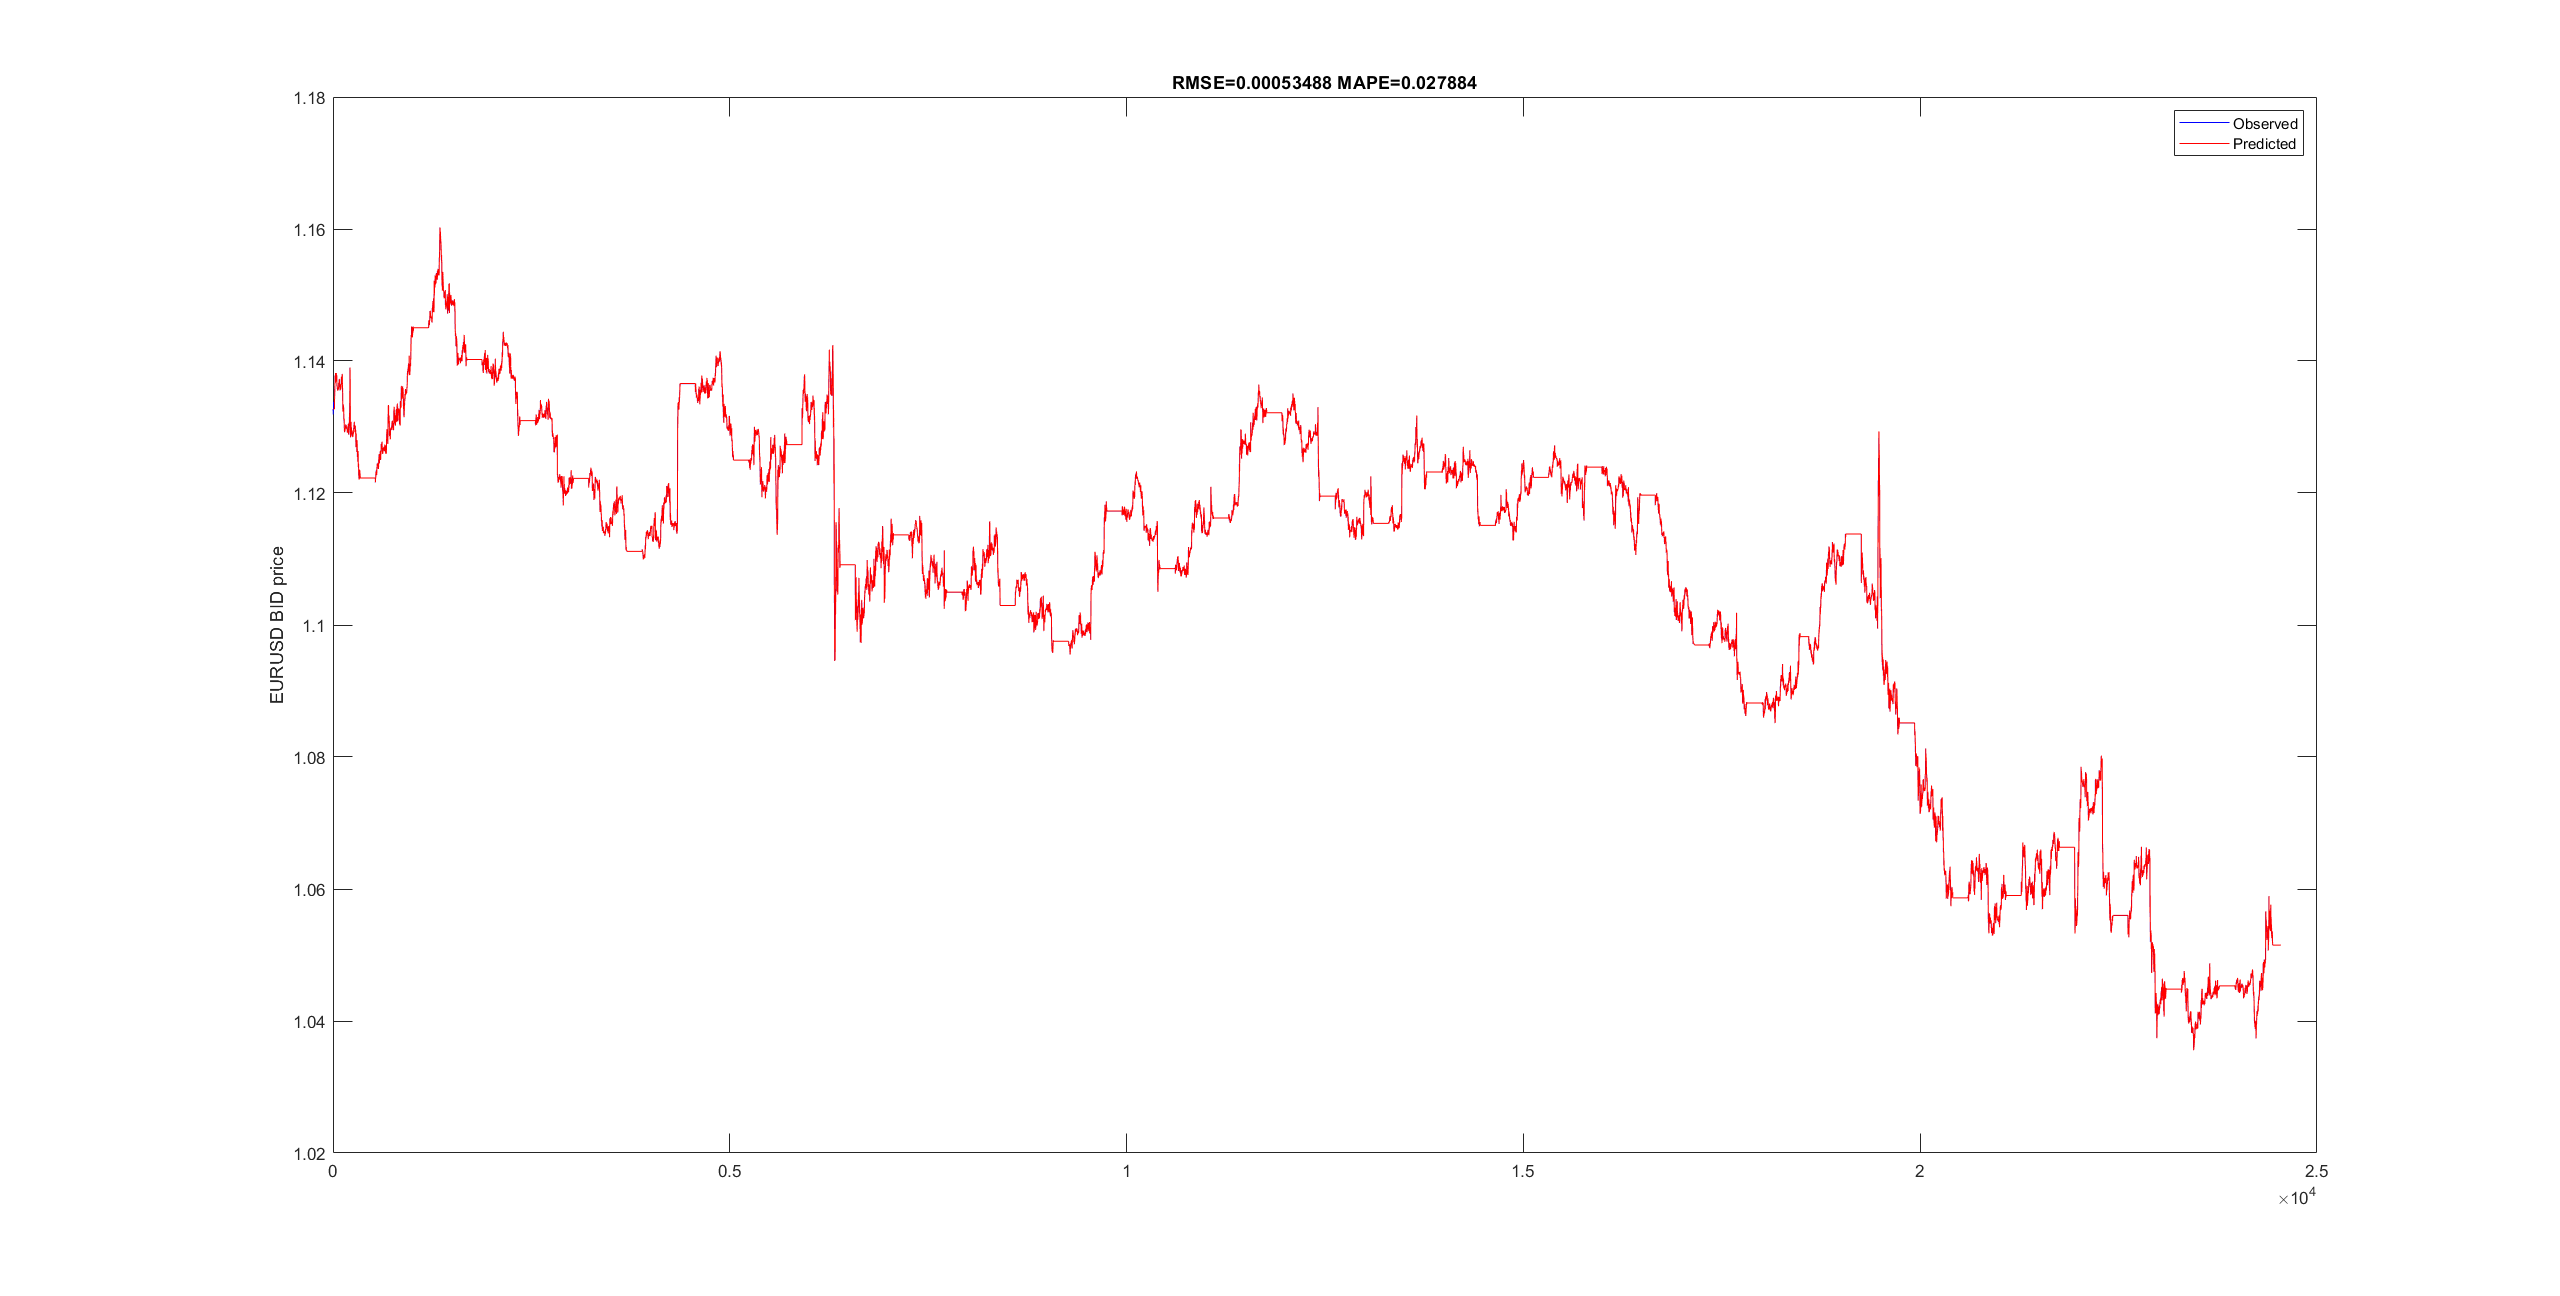
\includegraphics[width=\textwidth,keepaspectratio]{figs/arima_1_1_18_open.png}
  \caption{ARIMA(1,1,18) on Open price.}
\end{figure}

\begin{figure}[H]
  \centering
  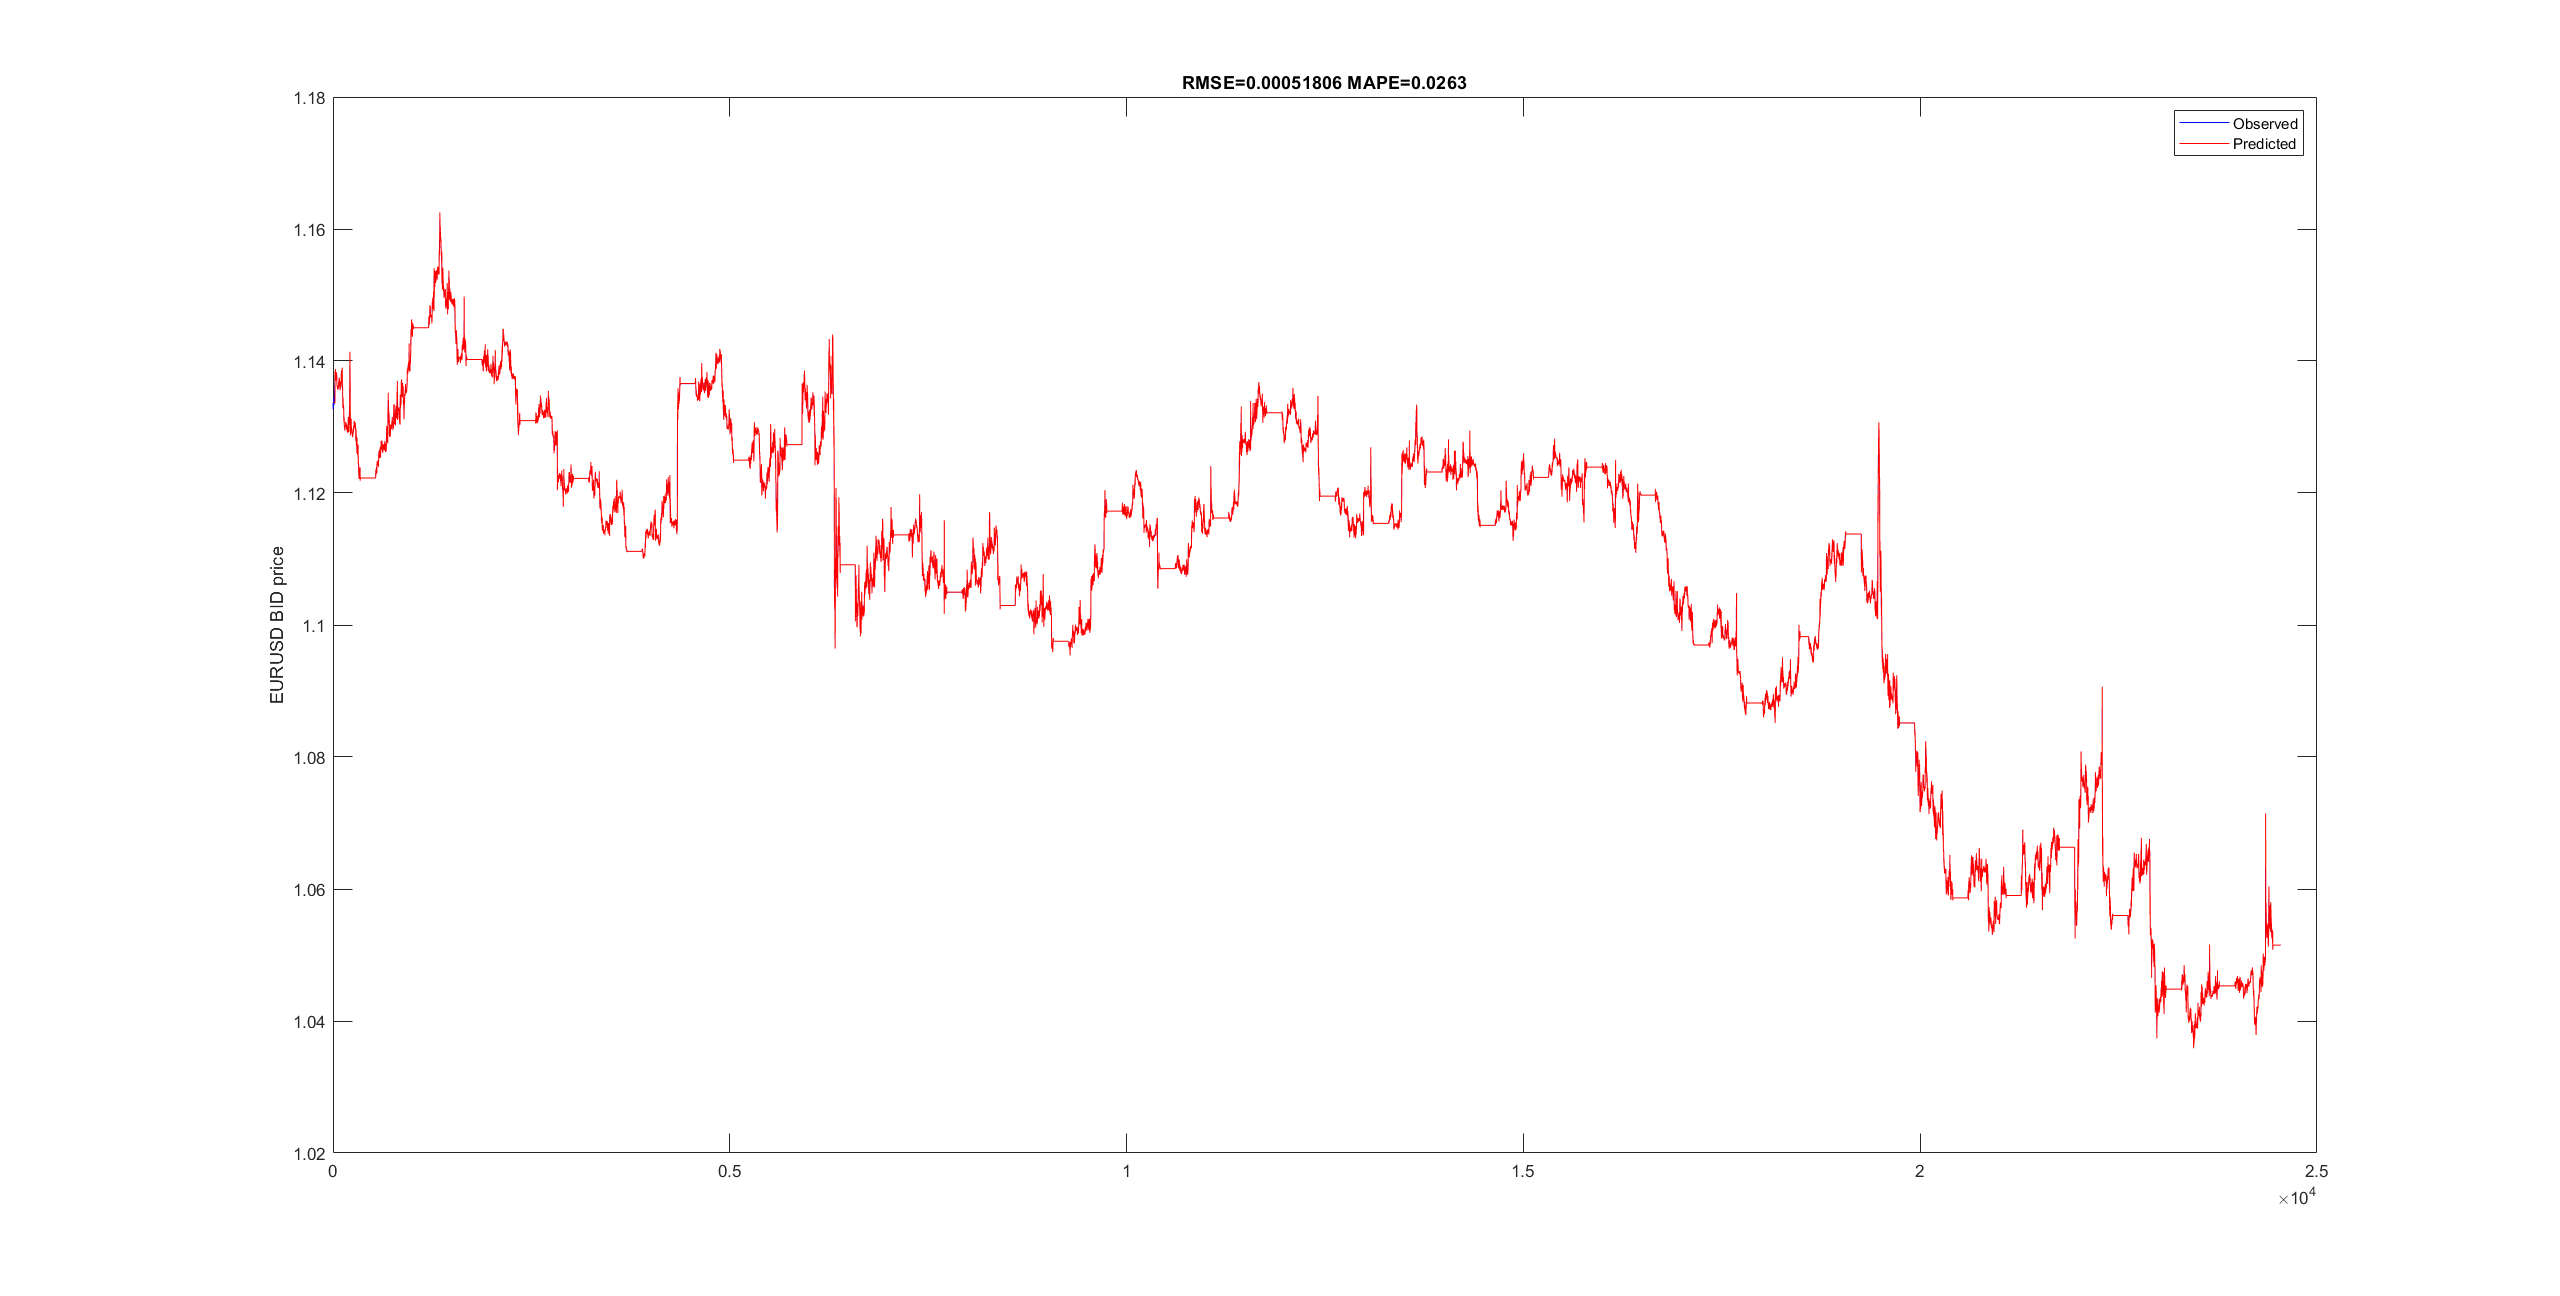
\includegraphics[width=\linewidth,keepaspectratio]{figs/arima_2_1_25_high.png}
  \caption{ARIMA(2,1,25) on High price.}
\end{figure}

\begin{figure}[H]
  \centering
  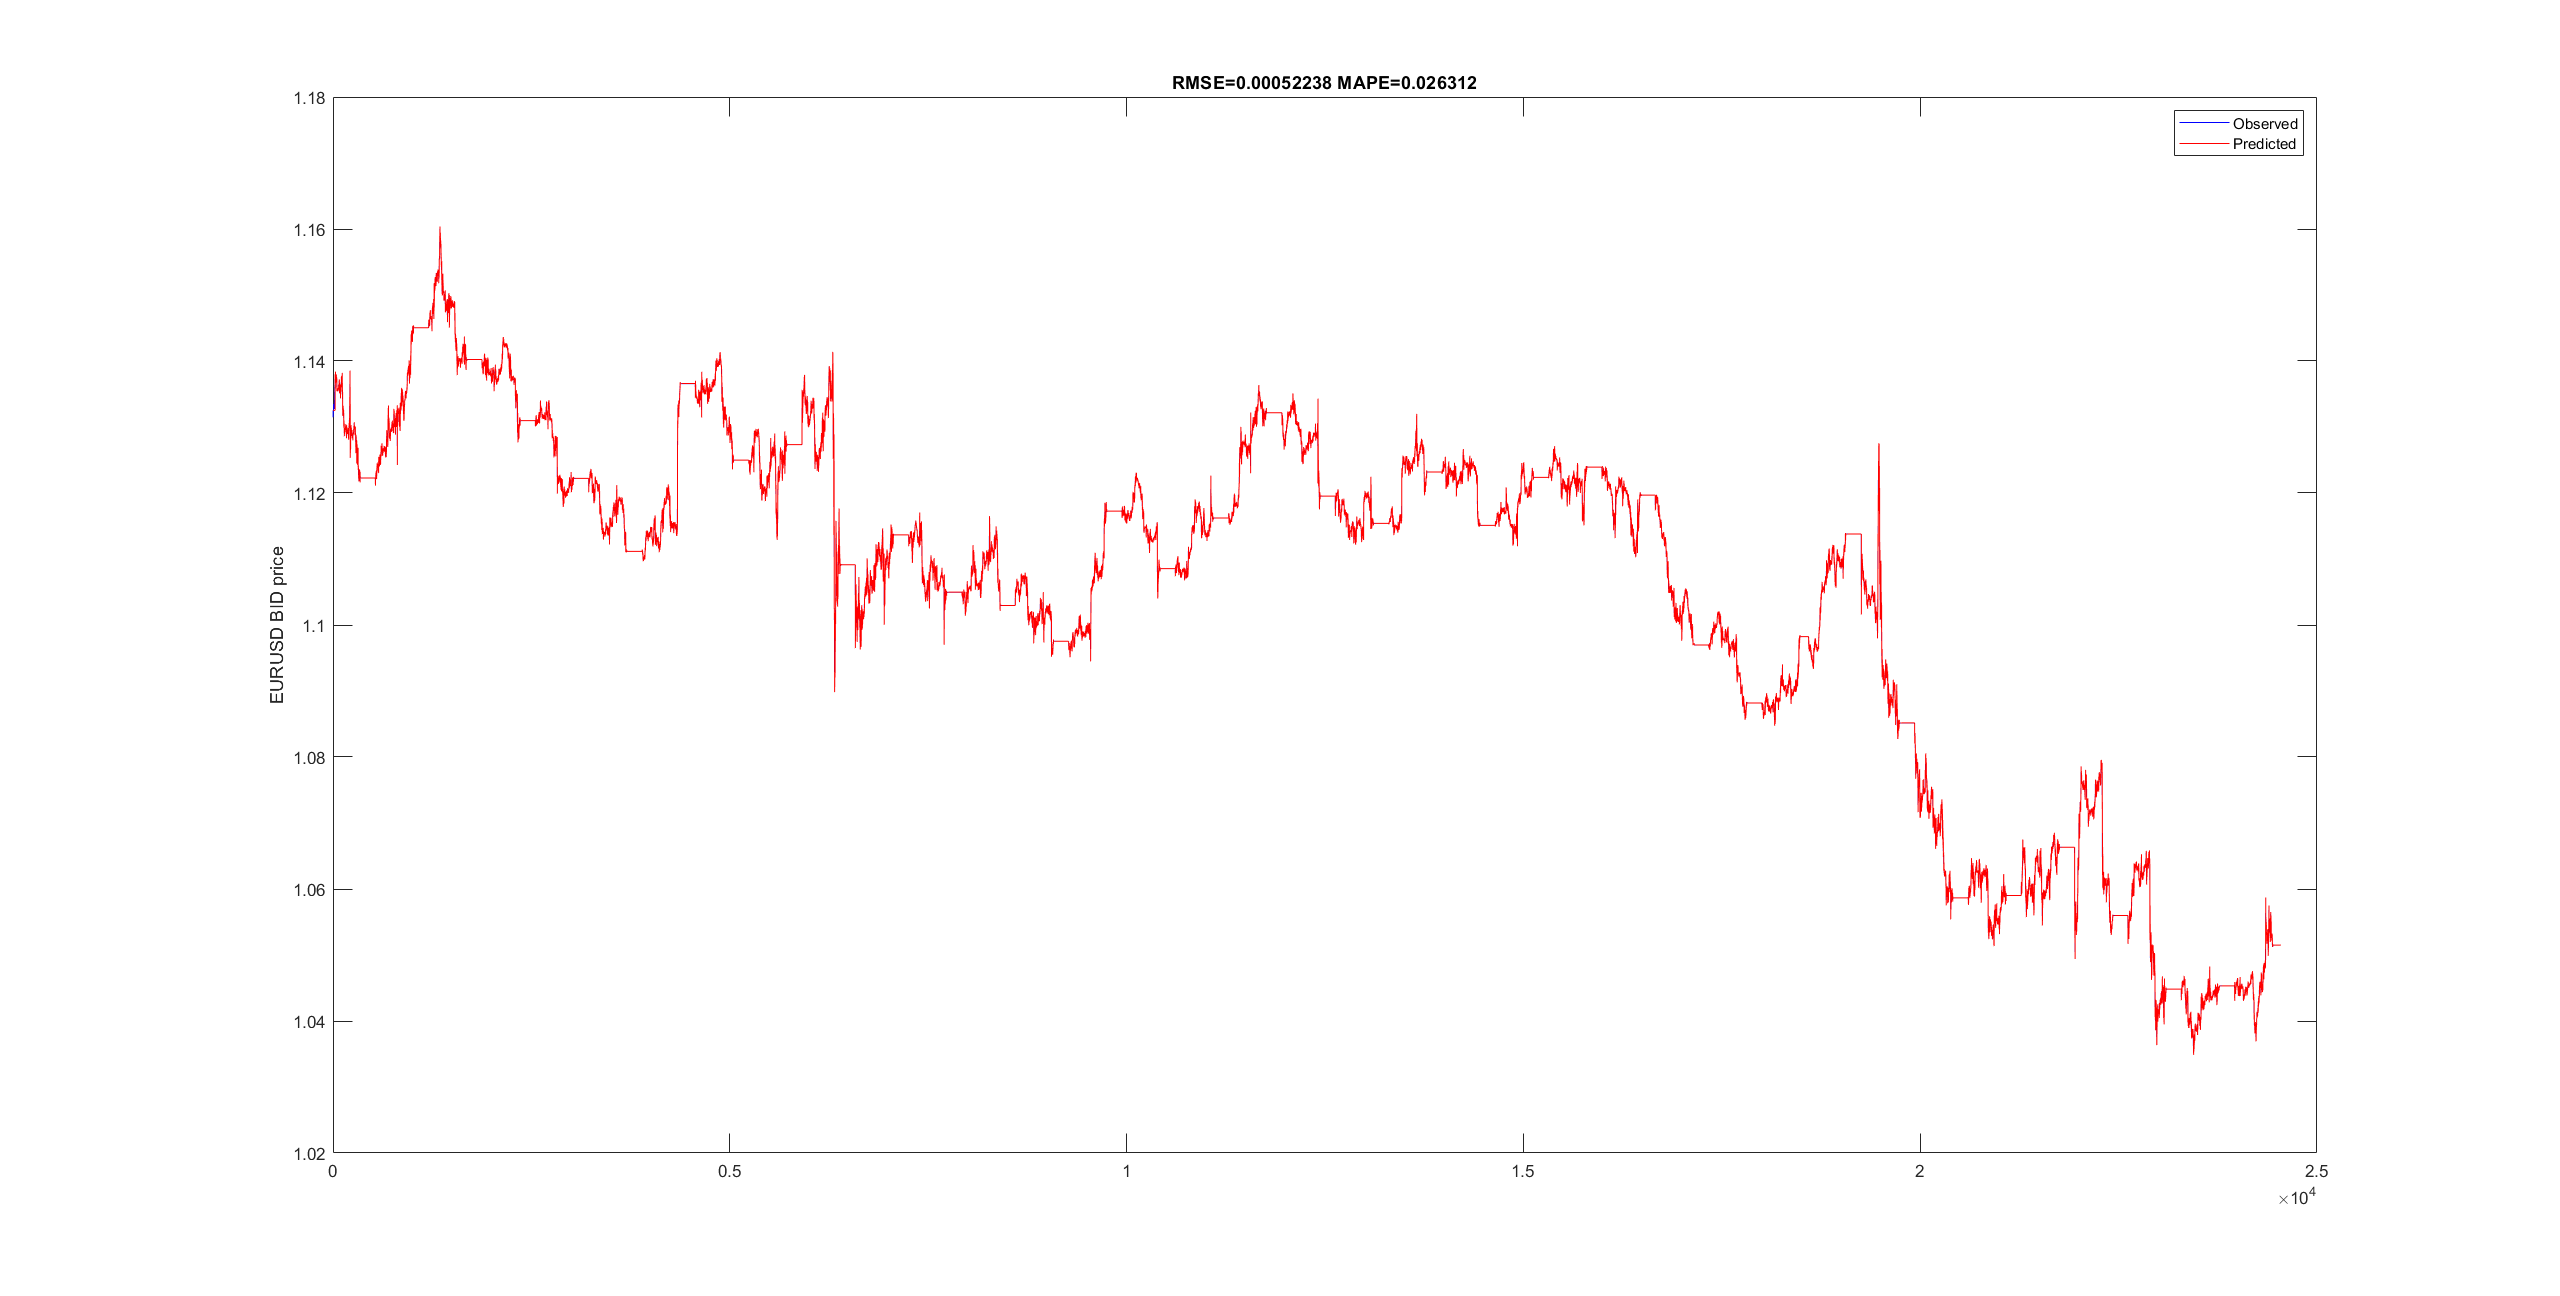
\includegraphics[width=\linewidth,keepaspectratio]{figs/arima_26_1_1_low.png}
  \caption{ARIMA(1,1,26) on Low price.}
\end{figure}

\begin{figure}[H]
  \centering
  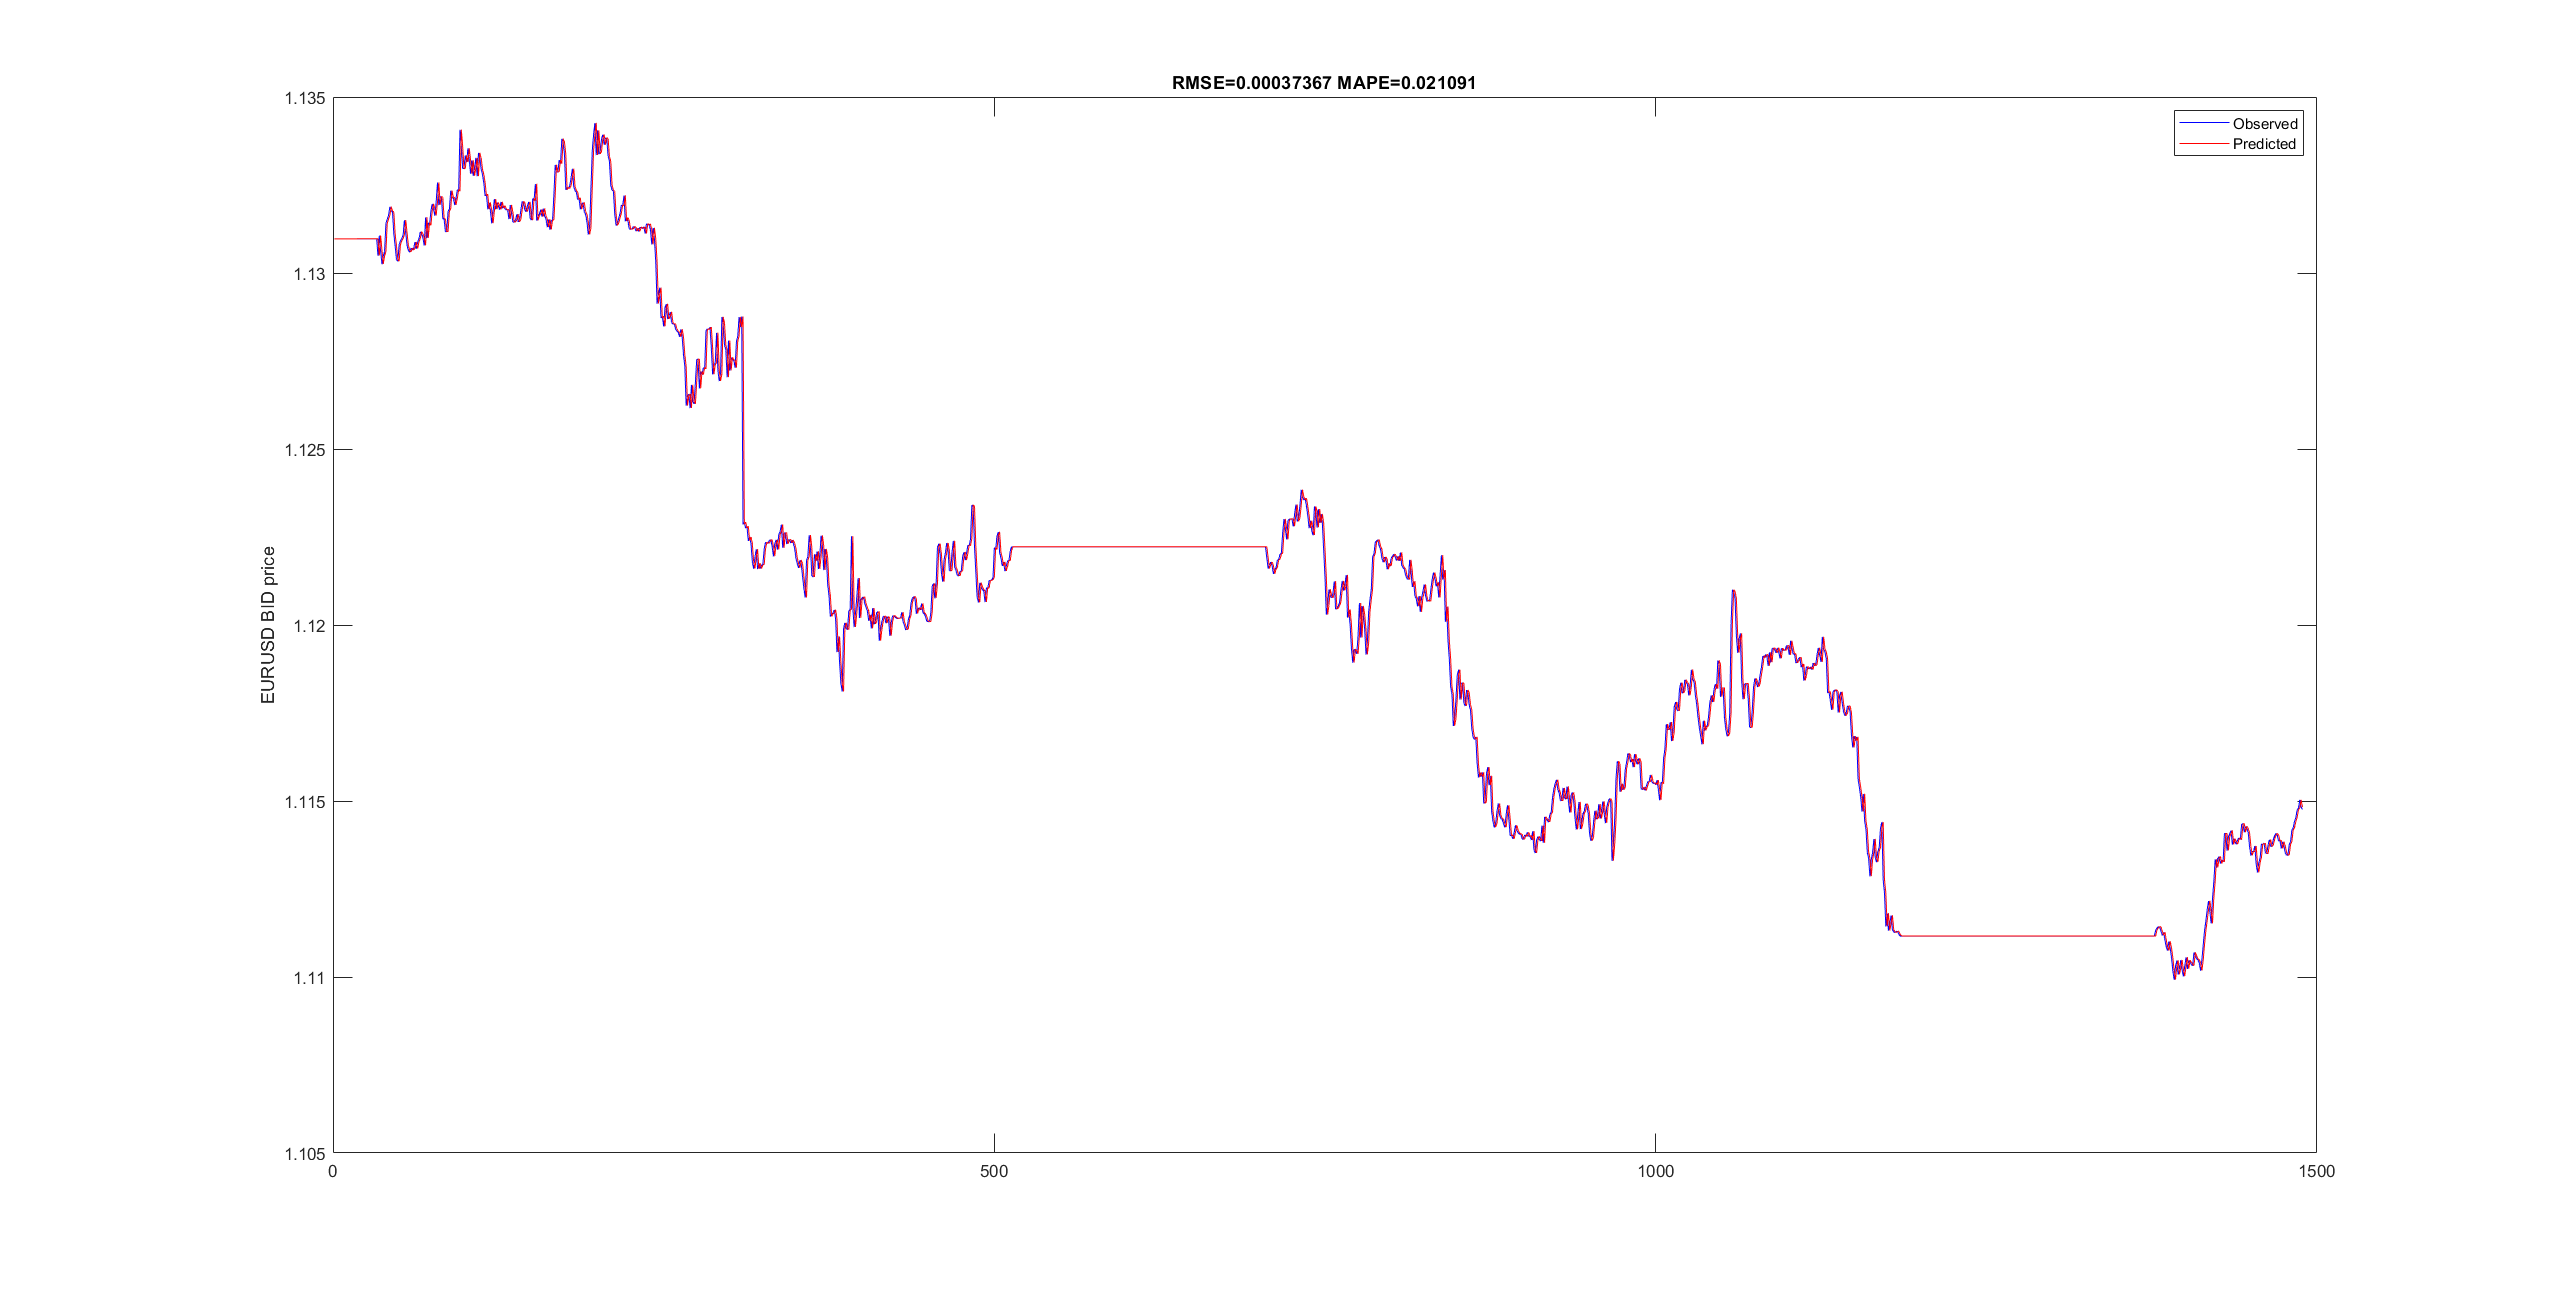
\includegraphics[width=\linewidth,keepaspectratio]{figs/arima_1_1_18_close.png}
  \caption{ARIMA(1,1,18) on Close price.}
\end{figure}


\subsection{VAR(p)}
\subsubsection{Model description}
VAR is applied to multivariate data. It is similar to $AR(p)$ model; however,
instead of considering $\{x_t\}$ as real values (univariate), we analyse
$\{\mathbf{x_t}\}$ as a timeseries of vectors $\mathbf{x_i}=(x_i^O, x_i^H, x_i^L, x_i^C)$. 

\subsubsection{Parameters selection}
Parameters selection for VAR consists only testing a range of lag with AIC. 

\subsubsection{Results}
Parameters selection algorithm gives the optimal parameter $P$ is 20 for the
train set. Since \textit{VAR(20)} fits the test set very well, for
visualization, we draw an additional plot for values 500-600 to highlights the
minute differences between prediction and actual observation.

\begin{table}[H]
\begin{tabular}{|l|l|l|l|l|}
  \hline
  P=20             & Open        & High       & Low        & Close      \\ \hline
  RMSE on Test set & 0.000377785 & 0.00035527 & 0.00036089 & 0.00037367 \\ \hline
  MAPE on Test set & 0.021241    & 0.019921   & 0.020236   & 0.021091   \\ \hline
  Overall MAPE     & \multicolumn{4}{c|}{0.00}                          \\ \hline
  Overall RMSE     & \multicolumn{4}{c|}{0.00}                          \\ \hline
\end{tabular}
\caption{Optimal parameters and error on Test set}
\end{table}

\begin{figure}[H]
    \begin{subfigure}[b]{0.5\textwidth}
      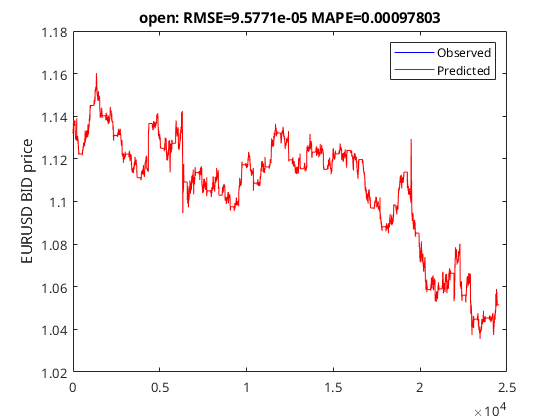
\includegraphics[width=\textwidth,keepaspectratio]{figs/var20open.png}
      \caption{Open}
    \end{subfigure}
    \quad\quad\quad\quad\quad\quad\quad
    \begin{subfigure}[b]{0.5\textwidth}
      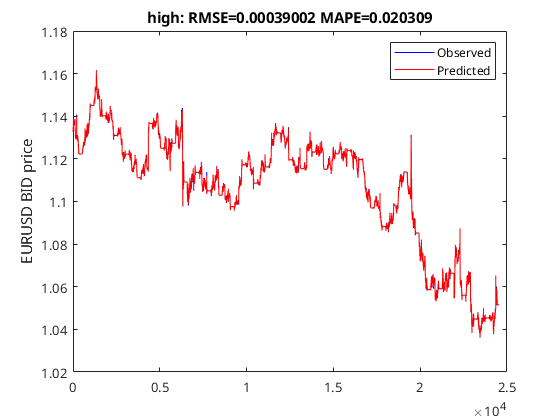
\includegraphics[width=\textwidth,keepaspectratio]{figs/var20high.png}
      \caption{High}
    \end{subfigure}\\
    \begin{subfigure}[b]{0.5\textwidth}
      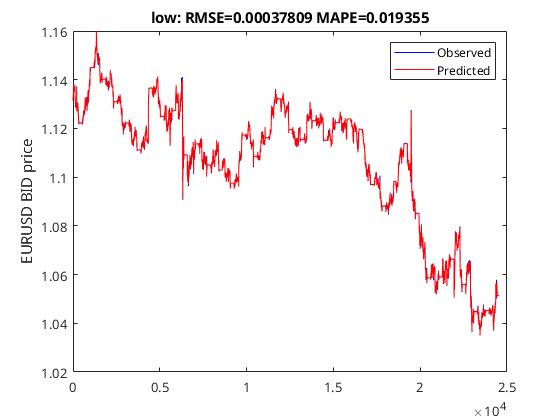
\includegraphics[width=\textwidth,keepaspectratio]{figs/var20low.png}
      \caption{Low}
    \end{subfigure}
    \quad\quad\quad\quad\quad\quad\quad
    \begin{subfigure}[b]{0.5\textwidth}
      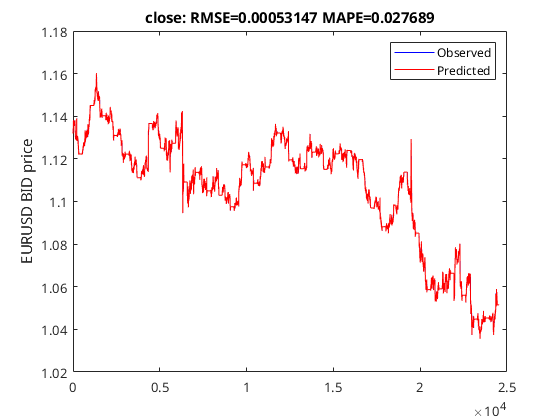
\includegraphics[width=\textwidth,keepaspectratio]{figs/var20close.png}
      \caption{Close}
    \end{subfigure}
    \caption{}
\end{figure}




%%%%%%%%%%%%%%%%%%%%%%%%%%%%%%%%%%%%%%%%%%%%%%%%%%%%%%%%%%%%%%%%%%%%%%%%%%%%%%%% 

\section{Deep Learning Model}
\subsection{Recurrent Neural Network}
Recurrent Neural Network (RNN) is introduced by \cite{rumelhart1988learning} to
process sequential input. In RNN, each state connects to the followed state to
form a directed graph. The structure of RNN makes it capable of handling
sequential data with temporal dynamic behaviour.
%% TODO graphics

Challenges in Recurrent Neural Network are \textit{vanishing gradient} and
\textit{exploding gradient}.

\subsection{Long-Short Term Memory}
Hochreiter and Schmidhuber (1997) \cite{gers1999learning} introduced Long-Short
Term Memory neural network architecture architecture to solve both vanishing
gradient and exploding gradient problem from RNN Cummins presented

\subsection{Proposed Network Topology}
Our survey on the data implies that significant autocorrelation may appears even
further than 20 timesteps into the past. In our proposed network topology, we

add more hidden units into each LSTM layers, so that the network can learn from
data points of higher lags.

\subsection{Experiments}
We consider using LSTM network in two experiments. In the first experiments, we
build and train the network to predict future values only by giving to history
lags of one timeseries \textit{(univariate)}. For example, we train the network to
predict one Open price value in the future given only the Open prices in the
past. This experiment is designed to compare the performance of LSTM with
$ARIMA(p, d, q)$ model.\\ 
In the second experiments, we build and train the network so that it would
predict one values ahead of one feature (e.g. one value of Open price ahead),
given history values of \textit{all} features in the past. This experiment is
designed to compare the performance of LSTM to $VAR(p)$ model.\\
In both experiments, since we want to predict the future values of all Open,
High, Low and Close features, we have to build and train one mode for each
feature accordingly. Therefore, in each experiment we have to build and train 4
models.

\subsection{Training}
As we can see from training progress, after the second epoch, the loss does not
decrease any more, meanwhile the 
\subsection{Results}

\subsubsection{Univariate}

\subsubsection{Multivariate}


%%%%%%%%%%%%%%%%%%%%%%%%%%%%%%%%%%%%%%%%%%%%%%%%%%%%%%%%%%%%%%%%%%%%%%%%%%%%%%%% 
\section{Conclusion}
As the results have shown, ...

However, computational effort spent for training LSTM deep learning model is
much higher than ARIMA and VAR. Furthermore the, adding components to neural network
topology results in higher computational cost. 

\pagebreak
\bibliographystyle{plain}
\bibliography{report}

\end{document}